\documentclass[12pt,a4paper]{article}
\usepackage{fullpage}

\usepackage{graphics}
\usepackage{color}
\usepackage[pdftex]{hyperref}
\usepackage{graphicx}
\usepackage{amssymb}
\usepackage{url}
\usepackage{multirow}
\usepackage{array}

\begin{document}

\title{A Survey of Physical Design Techniques of Information Systems}


\author{Karim Ali and Sarah Nadi\\
\{karim, snadi\}@cs.uwaterloo.ca \\
David R. Cheriton School of Computer Science\\
University of Waterloo\\
}

\date{}
% make the title area
\maketitle



\begin{abstract}
The physical design decisions taken during the database design lifecycle highly affect the database performance. These design decisions include the index
structures used,
which views can be materialized, how to partition the data etc. These decisions vary by the nature of the system being implemented. For example, the index
structures used for disk-based database systems differ from those used in a memory-based database system. In this survey, we present the elements of
physical design in different information systems. We start by describing the physical design of traditional disk-based relational database systems then compare
it to other types of information systems. Specifically, we look at the physical design of Main Memory Database Systems (MMDB), XML Databases, and Data
Warehouses. We examine how the specific nature of each of these systems affect its physical design. We focus on index structures, materialized views,
partitioning, and clustering.
\end{abstract}

\section{Introduction}

Relational Database Management Systems (RDBMS) have been the most popular type of Information Systems for decades. When we think of designing a database system,
we usually think of which data we need to keep track of and how will we properly organize it into meaningful tables. However, this is not the only phase in
database design. All of the designed tables need to be physically stored on disk. How these tables will be stored and accessed greatly affects the database
performance. Physical database design is concerned with the actual storage of data on disk. This means how the files are organized, and how they are accessed.
Data is stored in the form of records in files which reside on a physical disk. In this sense, we try to find the most efficient way possible to store and
access the data such that queries are answered and executed efficiently. In the traditional relational database system, this involved selecting proper indexing
techniques, partitioning the data for more efficient access, materializing the results of some queries, clustering and compressing the data, and many other
techniques \cite{finkelstein1988physical,lightstone2007physical}. The physical design aspects of relational databases have been studied in much detail. However,
over time, different types of Information Systems have emerged that have different characteristics. For example, most relational databases have been disk-based
where the primary copy of the data resides on disk. This is as opposed to Main Memory Relational Databases (MMDB) where the primary copy of the data resides in
main memory and no disk operations are needed to query the data. Such differences pose new requirements for the physical design of these systems.

This survey presents the different physical design patterns that have been used in different types of information systems. The systems discussed in this survey
are disk-based Relational Database Management Systems (RDBMS - traditional database systems), Main Memory Databases (MMDB), Data Warehouses, and XML
Databases. The aim of this survey
is not to explain the details of every data structure used in physical design, but rather to compare how the different data structures and techniques have been
used in these
systems. This includes explaining how alterations or additions are made to data structures to fit the specific needs of every system. Using the different
physical design methods used in disk based RDBMSs, we explore how these methods apply to the other systems and where the differences and similarities lie.

The rest of the survey is organized as follows. Section \ref{SEC-ELEMENTS} first explains different elements of physical database design used in traditional
disk-based databases. Section \ref{SEC-DIFFSYS} then discusses how each of the three other systems uses these elements, as applicable. Sections \ref{SEC-MMDB},
\ref{SEC-XML}, \ref{SEC-WAREHOUSES} discuss MMDBs, XML Databases, and Data Warehouses respectively. Throughout these sections, comparisons are
made as to how the different elements have been modified to fit the needs of each system. Section \ref{SEC-OPEN} mentions some of the currently researched open
problems in physical database design. Section \ref{SEC-CONCL} then summarizes and concludes this survey.

\section{Elements of Physical Database Design}
\label{SEC-ELEMENTS}

Relational Databases were first introduced by Codd \cite{codd1970relational}. Disk based Relational Database Management Systems (RDBMS) are the most common and
popular type of information systems. Since they have been extensively researched and have been around for many decades, we use them as the basis of our
comparison. In this section, we describe the different elements of physical design in RDBMS. These elements will also be examined in the other systems to see
how they apply to them.

\subsection{Index Structures}

The first physical database design decision to be considered is the choice of indices to be implemented. The concept of indices has been around for a long time.
Just like an index at the end of the book is provided to help find certain content faster, indices in an information system help find content in tables faster.
The main idea of an index is to have each record in a table have a unique identifier (primary key) and then organize these identifiers in a certain way that
allows for fast access of a specific record. Of course, indexing can be done on any column in the database and not necessarily the primary key. There are many
type of indices that have been used in information systems.

B-trees (short for Balanced Trees) are the most used database index structure.  The B-tree is essentially similar to the traditional Binary Search Tree, but
instead of having one value per node, a B-tree can have many values per node \cite{comer1979ubiquitous}. B-trees are suitable for relational databases since the
cost of retrieval in a B-tree is at most proportional to: $log_{d}\frac{n+1}{2}$. The cost of insertion and deletion is at most proportional to $log_{d}n$ due
to the possibility of progressing back up the tree to balance it after an insertion or a deletion. Although B-trees do well in retrieval, deletion and
insertion, they do not perform well in sequential search. 

Different variations of B-trees have been used. For example, B+trees are now the main method of indexing in current disk-based Relational Databases
\cite{lightstone2007physical} such as DB2, Oracle, and SQL Server. The main difference between the B+tree and the B-tree is that only the leaf nodes contain
data pointers in a B+tree, and leaf nodes contain pointers to each other as shown in Figure \ref{fig:b+tree}. In Prefix B+trees, instead of using the actual key
value of a record, a prefix from the key value is used to decrease the storage size needed which will in turn allow more records to be stored per node thus
decreasing the height of the tree. B+trees have been successful in relational databases since data is ultimately recorded in files. Since B+trees have a high
fanout, they allow less I/O operations to access a specific data record which is stored in a specific file.

Bitmap indices represent another type of index structures that is commonly used and cited in the literature. Using bitmaps as an index structure was first
implemented as part of the architecture of the Model 204 commercial database of Computer Corporation of America for the IBM 370 computer
\cite{patrick1987model}.
A bitmap index structure is based on a bitmap (i.e. bitset or bit array) data structure where individual bits correspond to values in unique records. Given a
table column $C$ where a record $x$ can have one of six unique values, a traditional bitmap index defined for $C$ generates one bitmap vector for each of the
six different values ($B0-B5$). If the value of $C$ for record $x$ is set to 3, the corresponding bit in vector $B3$ is set to 1. Otherwise the bit is set to 0.

\begin{figure}[!t]
\centering
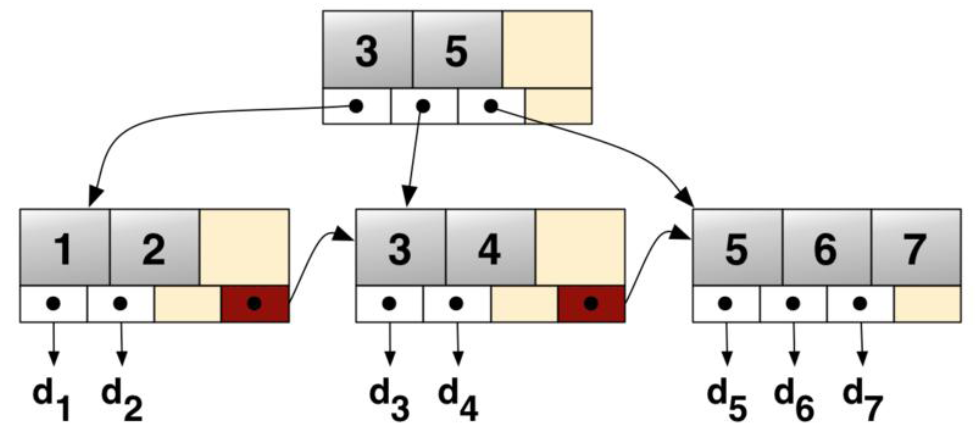
\includegraphics[width=7cm]{figs/b+tree.png}
\caption{B+tree}
\label{fig:b+tree}
\end{figure}

Bitmap indices are best used when the set of possible key values in the index is small with a large number of records, e.g. gender attribute
\cite{oneil1995multi}. Bitmap indices outperform B+trees for low cardinality attributes. The reason is that given an attribute with low cardinality, defining a
B+tree index
on it means that the tree will have very few leaf nodes, each one storing a very long list of record identifiers (RIDs). On the other hand, defining a
bitmap index on that same attribute means that such long lists or RIDs will not be stored, rather bit vectors that represent the distinct attribute values will
be stored as previously explained. This leads to a direct benefit of consuming less storage space. Moreover, queries in that case can be answered using bit-wise
logical operations (e.g. and, or, not) which can improve query performance \cite{oneil1997improved}. Another advantage of bitmap indices is the ability to
perform more
efficient joins by creating bitmap join indices and using those indices to calculate the result of the join \cite{oneil1995multi}. Although there are many
benefits
gained from using bitmap indices, they poorly perform during updates. The reason is that when an update is to be executed to a bitmap index, the whole bit
vector
for the index is locked, blocking any access to the index for other operations. The lock is then released when the update is done. That is why bitmap indices
are usually used for read-mostly databases, a famous example of which are data warehouses (Section \ref{SEC-WAREHOUSES}).

Another variation of indexing, a hash table index, often simply known as a hash index is used to organize unordered physical database tables for efficient
access \cite{lightstone2007physical}. This type of index is usually defined for keys that have unique values in the data records. Creating this index requires
passing the attribute (key) value to a hash function that maps it to a starting block address (i.e. bucket address). Afterwards, table insertions will be done
according to the hash function, as well as querying the records later.

In general, indices are a way of organizing the logical structure of a database without altering its physical structure. However, sometimes it is desirable to
store related records near each other on disk for better locality. This can be achieved through implementing a clustered index on the desired key values.
Otherwise, the created index is known as a non-clustered index. The primary advantage of a clustered index is therefore the ordering of the physical data rows
in accordance with the index blocks that point to them. Therefore, fewer data block reads are required to answer a given query. The only caveat with using a
clustered index is that there can only be one clustered index per table because the physical organization of the table must be fixed
\cite{lightstone2007physical}.

\subsection{Materialized Views}

In a large database system, there are usually a few complex queries that require the joining of many large tables. If these queries are frequently run, then the
database performance is likely to suffer, and users have to wait for a long time to get the results back. If we know these queries beforehand, it makes sense to
simply store the results of the queries on disk instead of recomputing them each time. Oracle 8i introduced materialized views to fit this purpose. By
precalculating the results of a complex query, and storing them in a table on disk, this new table containing the query results will be much
smaller than the original tables. This decreases I/O access costs and thus increases performance \cite{lightstone2007physical, chaudhuri1998overview}. Once a
materialized view exists, the user can either explicitly query the materialized view, or enter the original query, and have the query optimizer rewrite the
query to use the materialized views instead of the original tables. Many query optimization techniques have relied on rewriting queries using views (e.g.
\cite{levy1995answering, gupta1995aggregate, goldstein2001optimizing, abiteboul1998complexity}), but discussing the details of the rewriting process is beyond
the scope of this survey.

Despite the fact that materialized views provide a significant improvement in performance, we cannot simply create a materialized view for each frequent query.
First, materialized views consume disk storage which might be limited. The second, and main, problem with materialized views is their maintenance. Ensuring that
the views have the most up to date data is tricky, and may outset the benefit of using materialized views if it is not properly designed. Finally, having
several materialized views may increase the cost of searching for the appropriate view to use during the query optimization stage.

\subsection{Partitioning}

Partitioning in physical database design aims to reduct the workload on any one hardware component (E.g. an individual disk). This is achieved by partitioning
(dividing) the data over several disks \cite{lightstone2007physical}. There are two main categories of partitioning: horizontal partitioning and vertical
partitioning \cite{agrawal2004integrating}. Horizontal partitioning divides the table into sets of table rows where each row or record still has all the
attributes of the table \cite{ceri1982horizontal, shin1985partitioning}. For example, dividing the data by date where all data dating less than year 2000 lies
in one partition while all data dating more lies in another. On the other hand, vertical partitioning reduces the width of the dataset by storing some
attributes in one table, and some in another. Usually, less frequently queried columns are partitioned together to reduce the size of the table. We will see in
Section~\ref{SEC-WAREHOUSES} that vertical partitioning is frequently used in Data Warehouses where not all the columns of a table are analyzed for decision
support.

The main advantage of any type of partitioning is to reduce the amount of time it takes to scan a table which in turn improves performance
\cite{lightstone2007physical}. For example, if a table has 1000 records, and a query is only using the first 20 records then having these 20 records in a
partition containing 50 records will save time as opposed to examining all the 1000 records. Horizontal partitioning is more widely used, and is implemented in
all current DBMSes \cite{mysqlpartitioning, sqlsrvpartitioning, sybasepartitioning, postgrepartitioning, oraclepartitioning, db2partitioning} which explains
why there exists many flavors of horizontal partitioning techniques. There are three major types of horizontal partitioning: range partitioning
\cite{dewitt1986gamma}, list partitioning \cite{lightstone2007physical} (which is a variation of range partitioning), and hash partitioning
\cite{lightstone2007physical}. Of course, one can mix and match those partitioning schemes and come up with a composite partitioning that fits a particular
situation \cite{lightstone2007physical}. Table \ref{tab:horpartition} shows different categories of horizontal partitioning, and the situations they are suited
to. Combining partitioning and indexing can often lead to better performance. For example, if List partitioning is used to divide a table by regions and then a
bitmap index is used on that table, finding records in the same region or state can be much faster. Finally, partitioning is one of the important
methods used to achieve parallelism. Partitioning the data into different physical
devices to achieve parallelism when accessing it can greatly increase the performance of the database.

\begin{table}[!t]
\centering
\scalebox{0.7}{
 \begin{tabular}{p{1.8cm}||p{4cm}|p{3.6cm}|p{4cm}|p{5cm}}
& \textbf{Range Partitioning} & \textbf{List Partitioning} & \textbf{Hash Partitioning} & \textbf{Composite Partitioning}\\
\hline\hline
\textbf{How?} & If key falls in range & List of keys & Hash function& Hybrid\\
\hline
\textbf{Why?} & Disk limits & Group point values & Range/List are N/A & According to needs\\
\hline
\textbf{Benefits} & \multicolumn{4}{p{16cm}}{\centering Partition elimination \linebreak Improved administration \linebreak Fast roll-in/out \linebreak Implicit
clustering }\\
\hline
\textbf{Example} & %\begin{itemize} 
                    \raggedright - Zip code \linebreak
		    - Time range &
                  \raggedright
		    - Regions \linebreak
		    - States
		     & \raggedright
		    - EmployeeId \linebreak
		    - ProductId &
		    Hash then List \\
\hline
\textbf{RDBMS} & MySQL, DB2, Oracle, PostgreSQL, SQL Server & MySQL, Oracle, PostgreSQL, SQL Server & MySQL, Oracle & MySQL, Oracle\\
\end{tabular}
}
\caption{Types of horizontal partitioning}
\label{tab:horpartition}
\end{table}

\subsection{Clustering}
Clustering is the process of grouping related data together on disk for efficiency of access and maximizing resource utilization. Data clustering benefits from
the fact that sequential I/O access in physical disks is much cheaper than random access. Therefore, records that are likely to be queried together are
clustered (stored physically together) to decrease the number of random I/O accesses. Whenever the number of I/O random accesses is decreased, CPU blocks are
also reduced which result in an overall reduction of CPU costs improving the query performance, especially for multidimensional queries (e.g. group by)
\cite{lightstone2007physical}. The same concept of data clustering can similarly be applied to multiple dimensions (columns or column attributes) of a table.
Kennedy et al. \cite{kennedy2005} summarizes the benefits of multidimensional clustering as follows:

\begin{itemize}
 \item Dramatic reduction in I/O requirements due to clustering.
 \item Scans on any dimension index provide clustered data access.
 \item Dimensions/slices can be accessed independently using their block indexes.
 \item Block index scans can be combined (ANDed, ORed).
 \item Access to the clustered data is much faster.
\end{itemize}

On the other hand, defining clustering keys, clustering scheme, and the granularity of clustering is very difficult. Accordingly, the problem of
designing an optimal clustering scheme has combinatorial complexity, having an extremely large search space \cite{jagadish1999snakes}.

\subsection{Other Physical Design Techniques}

There are other physical design methods used to improve the performance of the information systems~\cite{lightstone2007physical}. For example, data compression
can
be used to make more data fit into a fixed amount of disk space such that it can be access faster. However, compression is only beneficial if the cost of
executing the compression algorithm is lower than the I/O cost of accessing the data. Otherwise, compressing the data might just add an overhead without
improving performance. Data striping is used to distribute data that is accessed together across multiple disks. This allows the data
to be retrieved faster through parallelism. Striping has the same goals as partitioning. However, striping is more geared towards the hardware level
which is beyond the control of the database while partitioning is within the control of the database. Database reliability is also improved through mirroring
which involves duplicating the data on multiple disks. Finally, refining the global schema to reflect query and transaction requirements is also sometimes used.
This is called denormalization which can be thought of as manual clustering of the data by hand to improve performance.

\section{Physical Design of Different Information Systems}
\label{SEC-DIFFSYS}

Given the different physical design methods explained in the previous section, we now look at how these methods apply to different types of information systems.
Mainly, how they apply to Main Memory Relational Database Systems (MMDB), Data Warehouses, and XML databases. We mainly focus
on the first four techniques discussed in Section~\ref{SEC-ELEMENTS} as these are the main design decisions involved in physical design.

\subsection{Main Memory Relational Database System (MMDB)}
\label{SEC-MMDB}

A Main Memory Database (MMDB) (sometimes referred to as in-memory database) is one where the primary copy of the data resides in the main memory of the system
rather than on a disk~\cite{garcia1992main}. It should be noted that this is different from caching. Disk-based database systems use the main memory to cache
query results. However, MMDB's primary copy of the data resides in main memory. Accessing data in main memory is faster than disk, and so MMDBs usually have
better performance that disk based systems. On the other hand, main memory is more expensive and the size is limited in comparison to disk. MMDBs are
essential to use when some of the collected data cannot, or will not, be stored on disk in the first place. For example, phone switch data may be needed for
reasoning with other stored data, but it is captured in real time and will not necessarily be stored on disk. MMDBs have many implementation challenges that
have been addressed throughout the research community. These challenges will be discussed throughout this section. 

\subsubsection{Index Structures}

Garcia-Molina and Salem~\cite{garcia1992main} mention data access methods as one of the main challenges involved in MMDBs. Two considerations are taken when
designing index structures for MMDB. The first is that the data resides in main memory and not on disk, and so many of the
considerations taken for I/O operations are no longer there. Instead of focusing on disk access and disk storage, the data structures for main memory
databases should focus on the efficient use of CPU cycles and memory~\cite{lehman1986study}. The second is having index structures cache conscious. Cache
memories improve performance by holding recently referenced data~\cite{smith1982cache}. If the memory reference is found in the cache, then execution proceeds
at processor speed. Otherwise, the data has to be fetched from main memory. With the big difference between processor speed and main memory speed, cache misses
are still relatively expensive. Lots of research work has shown that cache performance is very critical in MMDBs~\cite{boncz1999database,rao1999cache}. Thus, a
cache miss is still relatively expensive in main memory databases.
Accordingly, we will see that many of the index data structures proposed for MMDBs focused on being cache conscious or cache sensitive. In
summary, a main memory index should be able to reduce overall computation time while using as little memory as possible~\cite{lehman1986study}. It should also
be noted that unlike disk based systems where it is advantageous to store actual attribute values in the index, main memory systems do not require that.
Instead, pointers to the actual attribute values can be used. This, in turn, will reduce the size of the index which is preferable in this case.

In this section, we talk about three families of index structures used in MMDB: B-trees, T-trees, and Binary Search Trees. There are more recent index
structures developed for MMDB such as J+trees~\cite{luan2009prefetching}, but which have still not gained much popularity, and so we do not discuss them in our
survey. Table~\ref{tab:mmdbindexsumm} summarizes the features of the different index structures discussed in this section with respect to MMDBs. The T-tree is
the most used index for MMDBs (E.g. MySQL CLuster). However, there are other indexes used as well. For example, IBM's solidDB uses Trie (or prefix tree) for its
indexing. For their purposes, it served as a good index for main memory since it eliminates the need for many key comparisons~\cite{ibmsoliddb}.


 \begin{table}[t!]
\centering
\scalebox{0.8}{
\begin{tabular}{p{2.2cm}|p{6cm}|p{6cm}}
\hline
 \centering \textbf{Index Structure} & \textbf{Features} & \textbf{Cache Consciousness}\\
\hline\hline
B-tree & 
\raggedright -Good storage utilization \linebreak  \linebreak
\raggedright -Reasonably quick searching \linebreak \linebreak
-Fast updating 
& 
-Reasonable cache behavior if node fits in cache line\\
\hline
B+tree &
\raggedright -Reasonably quick searching \linebreak \linebreak
\raggedright -Fast updating
&
-Reasonable cache behavior if node fits in cache line\\
\hline
CSB+tree & 
-Same features of B+ Trees \linebreak \linebreak
-Stores child nodes in an array. Stores pointer to first child only and uses index calculation to get the rest
 &
-Good cache performance due to improved locality \& lower tree height (because of larger node size)\\
\hline

pB+tree & 
-Same features of B+ Trees
             &
-Improves cache miss performance by prefetching more data in each cache miss \linebreak \linebreak
-Node size is also increased leading to the same benefits of CSB+ Trees\\
\hline
T-tree &  
-Contains pointers to data values instead of the values themselves leading to better space utilization \linebreak \linebreak
-Many sorted keys per node \linebreak \linebreak
-Only minimum and maximum keys used for comparisons \linebreak \linebreak
\raggedright -Contains record pointers in every key \linebreak \linebreak
-Good update \& storage characteristics if Btrees.
             &
-Cache behavior was not considered at time of design \linebreak \linebreak
-Record pointers waste space in cache\\
\hline
CST & 
-Binary search tree for maximum value of each node leads to faster search \linebreak \linebreak
-More space efficient by removing pointers \& using array storage. Index calculation used to allocate values &
-Node size is aligned with cache line size to avoid misses \linebreak \linebreak
-Higher usage of cached data in binary search tree\\
\hline
CSS-trees & 
-Fast traversal in $log_{m+1}n$ ($m$ is the number of keys per node) \linebreak \linebreak
-Mainly suitable for read environments &
-Good cache behavior since $m$ is chosen to fit in the cache line size\\

\end{tabular}
}
\caption{Summary of index structures for Main Memory Databases (MMDB)}
\label{tab:mmdbindexsumm}
\end{table}

\subsubsection*{B-trees}
Although B-trees, explained in the previous section, are originally designed for disk based database systems, they were also found to be useful in
MMDB~\cite{lehman1986study}. In disk based systems, the B+ Tree is more used than the regular B Tree. However, in MMDBs, the B-tree would be
more suitable from a storage perspective since there is no gain from keeping all the data in the leaves. In a main memory system, this
would only waste space without improving performance. On the other hand, the B+ Tree uses multiple keys to search within a node. This means that
if the node fits in a cache line, this cache load can satisfy more than more comparison leading to better cache utilization~\cite{rao1999cache}. Additionally,
less data per node is stored in a B+tree which means there is better cache utilization. Therefore, B+trees in general have reasonable cache behavior, and
variations of them have been adapted in MMDBs.

However, the cache behavior of B+trees could still be improved. Therefore, Rao and Ross~\cite{rao2000making} propose the Cache Sensitive B+trees
(CSB+trees)~\cite{rao2000making} as an index structure for main memory. To do so, they eliminated most of the child pointers by storing the child nodes
in an array, and only keeping a pointed to the first child. Additionally, they used more keys in each
node to improve locality and reduce tree height~\cite{luan2009prefetching}. This also aligns the nodes size with the cache line size. Since the number of cache
misses in search operations is proportional to the height
of the tree, CSB+trees have fewer cache misses, and thus better performance.

Chen et al.~\cite{chen2001improving} propose using prefetching to improve the performance of B+trees. They call the new index structure prefetching B+tree
(pB+tree). Since current computer systems can prefetch different data simultaneously, the authors take advantage of this. The idea here is to increase the node
size of B+ Trees and employ prefectching at the same time. In a B+tree, every time we move down a level in the tree, a cache miss occurs. Accordingly,
prefetching larger sizes nodes means that we can overlap multiple cache misses before they occur. This is because in one cache miss, extra data is retrieved in
parallel with the originally requested data if it can be predicted sufficiently early. Figure~\ref{fig:prefetching} shows how prefetching retrieves the same
data in less time. This method, however, does not eliminate the full cache miss latency with every level in the tree.

\begin{figure}[!t]
\centering
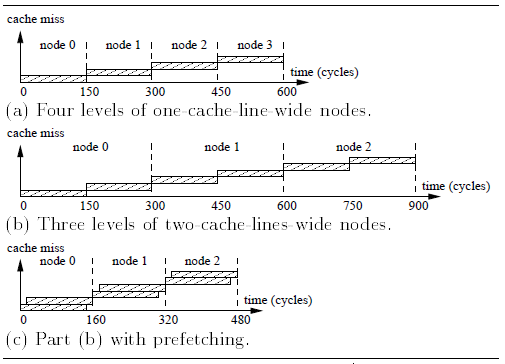
\includegraphics[width=7cm]{figs/prefetching.png}
\caption{Performance of various B+ Tree searches where a cache miss to memory takes 150 cycles and a subsequent access can begin 10 cycles
later~\cite{chen2001improving}}
\label{fig:prefetching}
\end{figure}

\subsubsection*{T Trees}
Lehmen and Carey~\cite{lehman1986study} introduce a new index structure, the T-tree, which combines the features from AVL Trees and B-trees that are suited to
main memory. Figure~\ref{fig:ttree} shows the proposed structure of the T-tree. They ran some experiments on data residing in main memory to compare the
performance of the T-tree to existing structures. All structures were modified to contain pointers to data values rather than the data values themselves. The
structures compared included  AVL Trees, simple arrays, B-trees, Chained Bucket Hashing, Extendible Hashing, Linear Hashing and Modified Linear Hashing. Their
experiments showed that for unordered data, Modified Linear Hashing gave the best performance, and for ordered data, T-trees gave the best performance for a mix
of searches, inserts and deletes. This is mainly because a T node contains many elements which results in good update and storage characteristics. The T-tree
was the first index structure specifically designed for main memory databases. The T-tree has many sorted keys per node, and only uses the minimum and maximum
keys for comparison. Additionally, every key contains a record pointer.



\begin{figure}[!t]
\centering
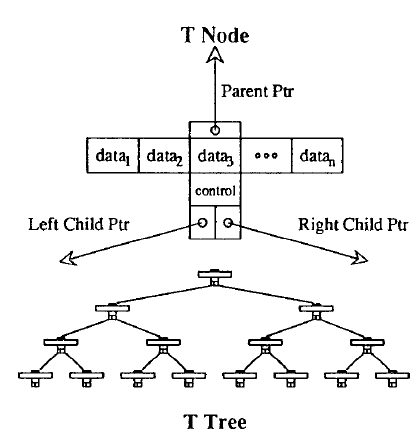
\includegraphics[width=7cm]{figs/Ttree.png}
\caption{T Tree by Lehmen and Carey~\cite{lehman1986study}}
\label{fig:ttree}
\end{figure}

Although T-trees have been specifically designed for MMDB, they did not consider the cache behavior at that time since the gap between processor speed and main
memory speed was not big then~\cite{rao1999cache}. Although many keys are
fit into one node, only the two end keys are used for comparison leading to low node utilization. Similarly, array binary search trees have the same problem. 
It was discovered that B+trees outperform
T-trees on modern processors because of the growth of cache miss latency relative to processor speed~\cite{rao1999cache,lee2007cst}. This is because the height
of the tree is high which makes the total number of memory accesses from the root to the leaf node higher. The other reason is that the node size is not aligned
with the cache line size. Another problem with T-trees is that there is a big waste of space in the cache because unnecessary data which is not used (the
record pointers) brought into the cache.

To resolve these issues, Lee et al.~\cite{lee2007cst} propose the Cache Sensitive T-trees (CST-trees). First, a binary
search tree whose node values are the maximum key of each node in the T Tree is constructed. That way, for a given value, the node containing this value could
be quickly located through searching the binary tree. Second, the need to store pointers is eliminated by storing the tree in an array and locating the
necessary nodes through index calculation. This produces a better utilization of the cache by removing the unused data. Finally, node sizes are aligned with
cache line size such that there are no cache misses when accessing data in each
binary search tree in the array.

\subsubsection*{Cache Sensitive Search Trees (CSS-Trees)}

Binary Search Trees have poor cache behavior when the array is much bigger than the cache. Rao and Ross~\cite{rao1999cache} propose the Cache Sensitive Search
Tree (CSS-tree) to improve this cache behavior. To do that, the search tree is stored as a directory in an array. The number of keys per node is chosen such
that the whole node fits in a cache line. This improves local searching within a node to just one cache miss. They also hard code the traversal within a node
such that finding the next node happens in $log_{m+1}n$ times rather than $log_{2}n$ times in a binary search tree where $m$ is the number of keys per node.
However, CSS-trees are only suitable for read environments since they eliminate nearly all child pointers, thus removing the support for incremental update.

\subsubsection{Materialized Views}
From our literature survey, it seems that materialized views are not frequently used in MMDB. This makes sense since the problems materialized views try to
address problems are not highly present in MMDB. That is, the cost of computing complicated join queries is much less in MMDB due to the low cost of accessing
the data in memory. Accordingly, the maintenance cost of materialized views in MMDB will outweigh their minimal benefit. However, this does not mean that they
cannot be used at all in MMDBs. As with all other physical design decisions, it rather depend on the query workload and the relative benefits of implementing
the technique. Accordingly, if the data is very large and may benefit from using materialized views, there is no reason not to use them.

\subsubsection{Partitioning}

Partitioning is used in disk based systems to divide the data into the physical pages in a way that will yield the best performance. This could be through
vertical partitioning or horizontal partitioning, as previously explained. In main memory databases, we do not have the issue of expensive disk access which
makes partitioning in memory unnecessary as it will not save any costs. However, partitioning is needed in the secondary storage of the data on
disk~\cite{gruenwald1990database}. Disk storage is still used as a backup of main memory databases. When a crash occurs, a reload of the database from disk or
archive memory takes place. In order to avoid page faults caused by referencing data that is still being reloaded, the reloading process must be designed to be
efficient in loading the important data such that the database users are not affected. An efficient MMDB reload takes into consideration the number of I/Os for
reload and the number of main memory references during transaction processing. Gruenwald and Eich~\cite{gruenwald1990database,gruenwald1990choosing} show that
horizontal partitioning is most suitable when the database performs more modifications than tuple deletions and more selections that projections and joins.
Vertical partitioning is chosen in the other cases. They also show that if we just concentrate on the reload performance (i.e the number of I/Os for
reload), then vertical partitioning is always the best choice. 


\subsubsection{Clustering}
Clustering in disk based systems is important because sequential I/O access is cheaper than random or dispersed I/O access. This is not the case with main
memory, and so clustering is not needed in MMDB~\cite{garcia1992main, moldovan2008databases}. Therefore, components of one object may be spread across memory
without impacting performance.

\subsection{XML Databases}
\label{SEC-XML}

XML (eXtensible Markup Language) is increasingly being used as a data exchange format. Accordingly, the ability to store and manage XML documents is needed.
Salminen and Tompa~\cite{salminen2001requirements} define an XML database as ``a collection of XML documents and their parts, maintained by a system
having capabilities to manage and control the collection itself and the information represented by that collection.'' Salminena and Tompa also highlight some of
the requirements of an XML database system. These requirements include querying parts of an XML document, and
transformations of XML documents. The main challenge in XML databases is path navigation since it is a very expensive operation.

There are two ways in which an XML database system can be designed. The first is to have the database internally translate the XML document into relational
tables (XML-enabled databases). The second is to have data structures that can persistently store XML documents (native XML databases). XML-enabled databases
are suited for data-centric documents which have a regular structure without any mixed content~\cite{bourret2003xml}. On the other hand, for document-centric
documents which have an irregular structure with lots of mixed content, having a native XML database is essential. Examples of XML-enabled databases include SQL
Server 2005 and Oracle, and examples of native XML databases include Tamino~\cite{taminodb},
eXist~\cite{meier2009exist}, and TIMBER~\cite{jagadish2002timber}.

In this section, we will discuss how the database's physical design needs to be adapted in both cases. Other challenges such as expressing and executing queries
and updates are faced in XML database design, but these are beyond the scope of this survey.



\subsubsection{Index Structures}

Despite the special nature of XML documents, the same index structures used in relational databases can still be utilized in XML databases. However, some
adjustments may need to be made to fit the nature of the XML documents. For XML-enabled databases, XML documents are usually represented as relational tables,
and then indexed similar to other tables. Pal et al.~\cite{pal2004indexing} describe how this is done in Microsoft SQL Server 2005. To start with, a new data
type called `XML' was introduced. This data type could contain values of complete XML documents, or just fragments of XML data. First, the different nodes in
the XML data are labeled with the ORDPATH~\cite{o2004ordpaths} mechanism. The XML data is then shredded into a relational table with five main columns: ORDPATH,
TAG, NODE\_TYPE, VALUE, and PATH\_ID. This information is then stored in a $B^{+}-tree$ as the primary index of the XML type. Additionally, a secondary index
can be created on any of the columns of the primary index to speed things up.


For native XML databases such as eXist~\cite{meier2009exist} or TIMBER~\cite{jagadish2002timber}, B+trees are still used to index the XML documents.
However, in contrast to XML-enabled databases, the XML data is not first stripped into a relational table. eXist uses a number schema to assign unique
identifiers to each node in the XML document. These unique number identifiers allow the determination of any node's parent, sibling or possible child nodes.
Four index files are created for XML data where all the indexes are based on $B^{+}-trees$. One index manages the collection hierarchy, one index collects nodes
in a paged file and associates unique node identifiers to the actual nodes, one index indexes elements and attributes, and the last index keeps track of word
occurrences and is used by the full text search extensions. Oracle uses a similar technique for indexing its XML content where an XMLIndex table is created for
XML entries~\cite{oracleXML}. This table contains a unique identifier for the XPath leading to the node, the row id of the table used to store the XML data,an
order key that identifies the hierarchal positioning of the node, a locater key used for fragment extraction, and the text value of the node.

TIMBER also uses a similar numbering schema. There are minor differences between the two numbering techniques, but the main idea is the same. The numbering is
based on three values of a node: its start label, its end label, and its level (i.e. nested depth). On the other hand, Sedna~\cite{taranov2010sedna} uses a
different reasoning to produce its numbering schema. Sedna assigns string identifiers to nodes such that they are lexically ordered according to the position
of the node. Despite the differences in the ways the numbering is constructed, it seems that existing indexing techniques can be adapted for XML databases. The
challenge is how to assign the nodes unique identifiers (the numbers or labels in the numbering schema) that can be used as identifiers in the index to
reflect the XML document structure. Additionally, in native XML databases, documents are usually grouped into collections, and an index may be used to search
within these collections. This is different from the node index which searches within a document.

Besides indexing the actual nodes, path indexing is also common in XML databases since usually queries search for a specific path which can be very expensive.
This is done by clustering together all the IDs of nodes on a given path, and creating an index for them~\cite{milo1999index, arion2008path}. Other techniques
include that proposed by Cooper et al.~\cite{cooper2001} where they propose an indexing mechanism for paths called ``Index Fabric''. An Index Fabric is based on
Patricia tries~\cite{knuth1998} which are used for string indexing, but is customized for disk-based systems. A path in an XML document is encoded into a unique
string, and is then inserted into the fabric. The encoded string is usually very short, and so searching is relatively fast.


\subsubsection{Materialized Views}

The main idea behind using materialized views is to rewrite queries using these views so that they run more efficiently. This is very important in XML
Databases since XQuery and XPath queries are complicated~\cite{arion2007structured}. Accordingly, materialized views are used in XML databases to improve
performance. The semi-structured nature of
XML data, and the expressiveness of most XML querying languages, view selection for optimization becomes a more complicated
problem~\cite{tang2009materialized}. Therefore, the choice of which views to materialize becomes more complicated in XML database. Much work has been
done on rewriting XML queries using views~\cite{arion2007structured, balmin2004framework, aouiche2006clustering, tang2008multiple}. However, this problem is not
within the scope this survey.

\subsubsection{Partitioning}
In XML-enabled databases, inlining during the shredding of the data such that children nodes that occur only once are stored with the parent node produces
better partitioned data~\cite{tatarinov2002storing}. Inlining shreds a document into sets of tables according to the document schema which leads to better
performance because queries tend to access less data. Such inlining is similar to horizontal partitioning~\cite{ramanath2003searching}. Additionally, it is
common to horizontally partition the mapped relational tables such that nodes of the same type are stored together~\cite{amer2002overview}.

\subsubsection{Clustering}
Clustering in XML databases follows the heuristic that sub-elements are likely to be queries with an element~\cite{jagadish2002timber}. Accordingly, elements
and their subelements are clustered together. In general, storing the XML data in document order it thought to be the best technique for efficient querying.
Additionally, Lian et al.~\cite{lian2004efficient} suggest clustering XML documents by structural similarity to produce more efficient access. This is done by
representing the documents as a structure graph (s-graph), and then identifying clusters based on similarity using a clustering algorithm.
Nayak~\cite{nayak2008fast} also proposes a similar clustering mechanism for XML data. Her technique is also based on structural similarity, but it is more
focused on the level structure of the XML documents.


\subsection{Data Warehouses}
\label{SEC-WAREHOUSES}
A data warehouse is a subject-oriented, integrated, time-variant, and non-volatile collection of data and decision support technologies, aimed at enabling the
knowledge worker (executive, manager, analyst) to make better and faster decisions \cite{inmon2002building, chaudhuri1997overview}. More than half of IT
executives named Data warehousing as the highest-priority post-millennium project for them \cite{sen2005comparison}. The value of data warehousing for an
organization depends on the organization's need for reliable, consolidated, unique and integrated reporting and analysis of its data, at different levels of
aggregation.

Data warehousing has been shown useful in many industries: manufacturing (for order shipment and customer support), retail (for user profiling and inventory
management), financial services (for claims analysis, risk analysis, credit card analysis, and fraud detection), transportation (for fleet management),
telecommunications (for call analysis and fraud detection), utilities (for power usage analysis), and healthcare (for outcomes analysis)
\cite{chaudhuri1997overview}.

Data warehouses tend to be extremely large, in fact it is quite possible for a data warehouse to store tens of petabytes of data while loading tens of terabytes
of data everyday \cite{thusoo2010data}. Datta et al. \cite {datta2002parallel} notes that the information in a data warehouse is usually multidimensional in
nature, requiring the capability to view the data from a variety of perspectives. Aggregated and summarized data become more crucial than detailed records in
such environment. Therefore, the workloads are query intensive with mostly ad hoc, complex queries, often requiring computationally expensive operations such as
scans, joins, and aggregation. Performing such operations on large amounts of data, like in the case of data warehousing, complicates the situation further.
Moreover, the results have to be delivered interactively to the business analyst using the system.

Although data in a data warehouse is extracted and loaded from multiple on-line transaction processing (OLTP) data sources (including DB2, Oracle, IMS
databases, and flat files) using Extract, Transfer, and Load (ETL) tools (Figure \ref{fig:dw}), a data warehouse is usually maintained seperately from the
organization's operational databases \cite{sen2005comparison, chaudhuri1997overview}. This architecture can be justified owing to the fact that operational
databases are finely tuned to satisfy known OLTP requirements and functionalities which are quite different from that of on-line analytical processing (OLAP)
which is supported by data warehousing. Analyzing data for decision support usually requires consolidating data from many heterogeneous sources of varying
quality, or use inconsistent representations, codes and formats. Moreover, understanding trends or making predictions requires historical data, whereas
operational databases store only current data. In OLAP, there's a need to support multidimensional data models and operations which requires special data
organization, access methods, and implementation methods, not generally provided by DBMSs targeted for OLTP \cite{chaudhuri1997overview}. Finally, in data
warehousing, query throughput and response times are more important than transaction throughput which is the major performance metric for operational databases.

\begin{figure}[!t]
\centering
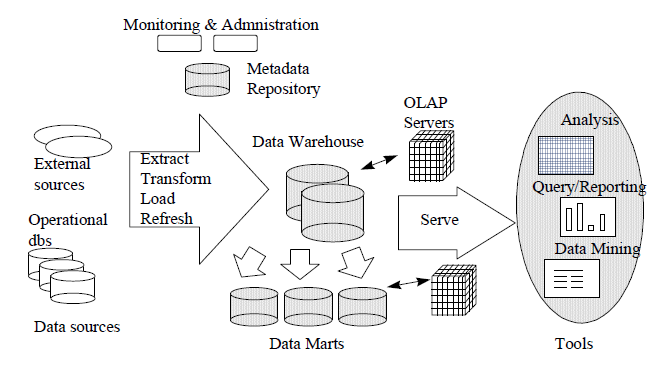
\includegraphics[width=9cm]{figs/dw.png}
\caption{Data Warehousing Architecture \cite{chaudhuri1997overview}}
\label{fig:dw}
\end{figure}

The design of a data warehouse can follow one of two paradigms: relational-based OLAP (ROLAP) or multidimensional OLAP (MOLAP). In ROLAP, data is stored in
relational databases and the support for multidimensional data is achieved through the use of the star schema \cite{cheung2001towards}. A star schema (Figure
\ref{fig:starschema}) is a database schema where a fact table $T$ that holds the base data in the database. Other tables in the database are dimensions for
table $T$, where each dimension table is linked to the fact table through foreign keys in $T$ pointing to the primary keys in the dimension tables. Thus, the
fact table, which is always the largest table in such schema, participates in almost all join operations \cite{datta2002parallel}. This might enforce some
design decisions for which indices to use, whether materialized views should be implemented to reduce the overhead of such expensive join operation or not. In
MOLAP, multidimensional data is directly stored in special data structures (arrays) forming data cubes where each side of the cube reflect a dimension of the
base data. OLAP operations are implemented on top of these special data structures. Usually a snowflake schema \cite{kimball2009data} or fact constellations are
used to logically design the data warehouse.

The rest of this section will discuss how such challenges and requirements of data warehouse design affect the selection of physical design elements during the
design process.

\begin{figure}[!t]
\centering
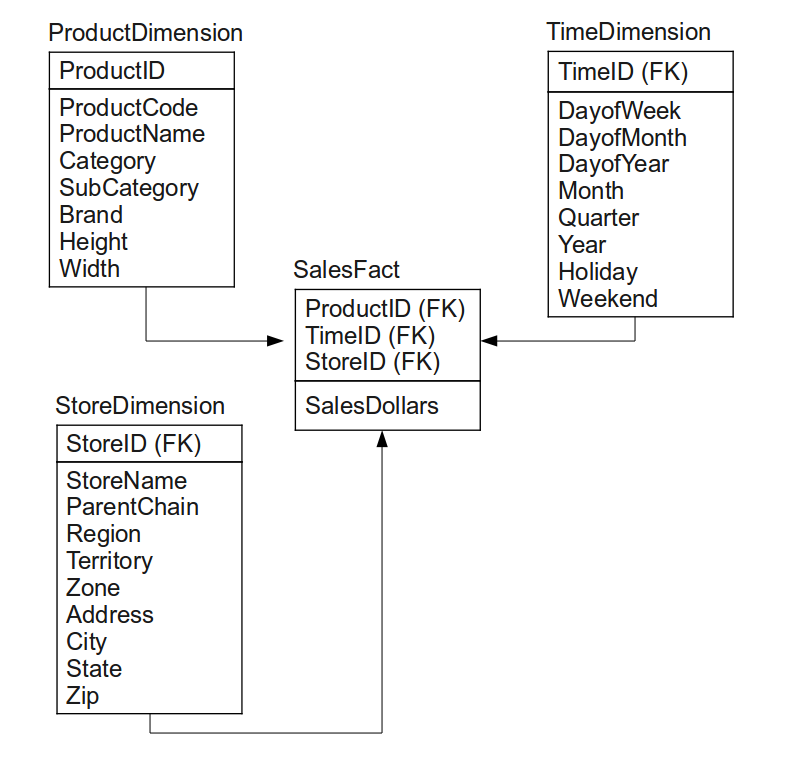
\includegraphics[width=9cm]{figs/starschema.png}
\caption{An example of a star schema}
\label{fig:starschema}
\end{figure}

\subsubsection{Index Structures}
Despite the design challenges involved in data warehousing, some relational index structures are still used after adapting them to match those challenges. 

\paragraph{Tree-based Indices}
The widely used B-trees have been modified to suit the requirements of a data warehouse design, such modification resulted in various tree-based indices:
UB-trees, BV-trees, K-D-B-trees, and R-trees. A UB-tree index \cite{bayer1997universal} is a variation of B+trees where support for multidimensional data is
provided by linearizing such data to be able to store it in one dimension. Usually the Z-order (Morton-order) \cite{morton1966computer} is used to perform this
type of linearization. UB-trees inherit the advantages of B+trees, so they are well suited for high cardinality attributes. They are also excellent for point
and interval queries (using the pointer in each leaf node to the next leaf node for faster index traversal). UB-trees also inherit the disadvantages of
B+trees. Therefore, they poorly perform for low cardinality attributes.

A BV-tree \cite{freeston1995general} is an unbalanced tree that maintains the characteristics of the B-tree in $n$ dimensions, and it can be degenerated to a
balanced tree in the one-dimensional case. A BV-tree index was an attempt to solve the problem of generalizing the characteristics of a B-tree index in $n$
dimensions. However, this type of indices did not really catch up in the literature of data warehouses since it has a very grave disadvantage. The
design of a BV-tree index suggests that the size of the index can span multiple-page for very large files (which is the case in data warehouses). Since
searching a BV-tree index might involve backtracking \cite{freeston1995general}, such property is not desirable.

K-D-B-trees \cite{robinson1981kdb} is another type of tree-based indices that tries to combine the multidimensional search efficiency of K-D-trees
\cite{bentley1975multidimensional} and the I/O efficiency of B-trees \cite{bayer1970organization}.

Another widely used tree-based index is R-tree \cite{guttman1984rtrees}. An R-tree is an extension of a B-tree with index records in its leaf nodes
containing pointers to data objects. Nodes in an R-tree correspond to disk pages if the index is disk-resident. The structure of an R-tree is designed so that a
spatial search requires visiting only a small number of nodes. The index is completely dynamic; inserts and deletes can be intermixed with searches and no
periodic reorganization is required. R-trees support multidimensional spaces by storing an n-dimensional rectangle, which is the bounding box of the spatial
object indexed, in the index record entries \cite{guttman1984rtrees}. R-trees were extended by Norbert et al \cite{norbert1990rstree} by designing the R*-tree
to support both sparse and dense data at the same time with a slightly higher cost (during insertion) than R-trees. Cheung et al. \cite{cheung2001towards}
describe how R-trees can be used to index dense data regions (MOLAP data cubes), while having pointers from the leaf nodes to sparse data points (ROLAP).

\paragraph{Bitmap Join Index}
Bitmap join indices are another widely used type of indices in data warehouses epecially when a star schema is used. A bitmap join index is simply a bitmap
index that is used for calculating the product of the join of the dimension tables. The result is then joined with the fact table to answer the given query
\cite{oneil1995multi}. In fact such process is less costly than joining the fact table with the dimension tables right away. The reason is that the fact table
is usually larger than the product of the dimension tables. The disadvantage of bitmap join being not amenable to index updates is not really applicable to the
case of data warehousing since a data warehouse can be considered as a read-mostly database.

\paragraph{Projection Index}
Not all columns in a data warehouse are of interest to the given query workloads. Therefore, it makes sense to have faster access to the columns that are used
the most to improve the query performance. That is why Projection indices are often used in data warehousing. A projection index involves positional indexing
of a column (form of vertical partitioning) where tuples are accessed based on their ordinal position \cite{datta2002parallel}. More results per I/O operation
is a direct benefit of using projection indices, since only data of interest are accessed and retrieved. However, only raw data can be fetched (e.g. column
list in a selection clause). A projection index can be further extended into a bit-sliced index \cite{oneil1997improved} where the projection index is sliced
vertically into columns of bits. Each column is a bit-sliced index. Bit-sliced indices can help reduce storage costs by using a number of bits per value which
is not a power of 2. For example, a SALES column contains all sales made in the last month, in pennies. Assuming no item cost more than $2^{20} - 1$ pennies (=
\$10485.75), this is 20 bit-slice indices). Moreover, computing aggregates, checking predicates can be done using efficient base-2 arithmetic operation. This
greatly enhances query performance since aggregates are crucial for data warehouses.

\subsubsection{Materialized Views}
A data warehouse must be built with a solid foundation that is flexible enough and responsive to business changes over time \cite{armstrong1997data}. Meanwhile,
a data warehouse can be seen as a set of materialized views defined over the remote data sources (Figure \ref{fig:dw}). That is why selection of materialized
views is one of the most challenging problems that faces data warehouse architects \cite{theodoratos2000general}. Most of the solutions in the literature
defined the problem of selecting views to materialize as \textquotedblleft selecting views for materialization in order to satisfy a number of design goals
given a set of constraints \textquotedblright. The problem can be reduced to a cost minimization problem, whether it is the query evaluation cost
\cite{harinarayan1996implementing}, total view maintenance cost \cite{kenneth1996materialized}, both \cite{yang1997algorithms}, or the operational cost
\cite{elena1997materialized, gupta2005selection, theodoratos1999designing, theodoratos1997data, theodoratos1999designingdw, theodoratos2000incremental,
yang1997algorithms}. Although materialized views greatly improves the performance of a data warehouse, it might not be as useful when the query workload is
formed of ad-hoc complex queries.

\subsubsection{Partitioning}
Both horizontal and vertical partitioning are heavily used in data warehouse design. Partitioning a data warehouse has many advantages. Horizontal partitioning
is usually used in data warehouses to make the job of the data warehouse administrators easier by facilitating the process of manages such large data
sources from which a data warehouse gets its data. In other words, it breaks down the management of large databases to managing smaller sets (i.e. partitions)
of data \cite{thusoo2010data}. More importantly, partitioning provides parallelism in various situations: loading data sources \cite{barclay1994loading},
performing parallel joins on huge data \cite{datta2002parallel}, faster drill-down and roll-up operations \cite{chaudhuri1997overview}. Partitioning also
facilitates compressing data that is not of interest to users of the data warehouse. Vertical paritioning is also used to keep seldom used columns away from
the process of answering queries for better performance.

On the other hand, if partitioning is over-used in a data warehouse, managing them will be a complex process due to the fact of having a huge amount of data.
Finally, there is an inherent cost of managing the meta data (e.g. data cube definition) when the number of partitions increases.

\subsubsection{Clustering}
A data warehouse is clustered by nature as Figure \ref{fig:dw} suggests. The data loaded into a data warehouse comes from various operational data sources,
each source has the data that is the most interesting/related to it (i.e. clustering). The data warehouse can be further divided into a collection of
conforming data marts \cite{sen2005comparison}. Each data mart stores data that is related to each other (e.g. based on the organization's business processes).
For example, one data mart can store sales data that is of particular interest to the Sales Department in an organization. Along with sales data,
product-related information can also be stored to provide better locality for queries that usually ask question about sales and products, and so on.

\section{Open Research Problems in Physical Database Design}
\label{SEC-OPEN}

Automating the physical database design choices has been a very attractive area of research that is still receiving lots of attention until now. Choosing which
indexes to create, which views to materialize, and how to partition data are hard choices. They are highly dependent on the schema used as well
as the query workload. The number of combinations of choices that can be made is very large making this task quite tedious and difficult for database
administrators. Accordingly, researchers have been inclined to find ways to automate these decisions. There were many early research efforts done in this
area(E.g. \cite{finkelstein1988physical, hammer76selec, frank1992selec, chaudhuri1997overview, schiefer1999db2, valentin2000select}), but most of these efforts
focused on having a static workload. Accordingly, research shifted to more dynamic ways to automate physical design. Initial attempts used an dynamic, on-line
approaches(E.g. \cite{bruno2007online, sattler2003, schnaitter2007}) where they observed the changes in the workload and adjusted the design accordingly while
attempting to predict future behavior based on the observed behavior. To avoid the problems of on-line design, researchers are also currently looking at how to
perform this dynamic physical design off-line (E.g. \cite{hannes2008,agrawal2006}). Additionally, finding better evaluation techniques to compare different
automatic physical design decision is currently being studied \cite{gebaly2008}.

Other problems which are currently being researched include improving I/O operations in database systems by using Solid State Drives (SSD) instead of of Hard
Disk Drives (HDD) \cite{lee2009, du2009, lee2008}. SSDs have faster read performance, but perform poorly in random writes. However, for certain applications in
databases and for databases where random writes are not as frequent, SSDs might be suitable. Using SDDs also seems promising when used for
transaction logs, and intermediate results of sorting and joining \cite{lee2008}.

Just like all other research areas are moving to the cloud, database systems are moving there too. Accordingly, lots of current research focuses on adapting
storage techniques and index structures to the cloud. For example, Wang et al. propose a new index structure for indexing multi-dimensional data in the
cloud \cite{wang2010indexing}. Lots of work is currently being done in this area. For example, Wu et al. \cite{wu2010efficient} propose a modified B+tree index
for datasets stored in each compute node. The exact requirements and solutions for data management in the cloud are still being
researched \cite{abadi2009data}, and so this is an area that is expected to receive more attention in the future as cloud computing becomes more prevalent.

This is by no means an exhaustive list of the problems still being researched in physical database design, but they provide a flavor of the challenges still
being faced. As shown, as new technologies such as SSDs or cloud computing environments emerge, database systems will need to adapt themselves to either make
use of them or to be able to cope with the new requirements they pose.

\section{Conclusions}
\label{SEC-CONCL}

In this survey, we present four elements of physical design in database: index structures, materialized views, partitioning, and clustering. We started out
by explaining how these design factors are implemented in traditional Relational Database Management Systems (RDBMS), and then presented how they are used in
other information systems. We focused on three types of information systems: Main Memory Database Systems (MMDB), XML Databases, and Data Warehouses. We
presented the challenges involved with each type of system, and how each of the four physical design elements were adapted or utilized to overcome these
challenges. Table \ref{tab:summary} summarizes the results of our survey. From our literature review, we found that the B+tree is the most utilized index
structure, and has been adapted and customized to fit the different needs of other systems. For example, it was made more cache conscious to fit MMDB needs,
and was changed to apply to multidimensions to fit the Data Warehouses needs. Materialized views were found to be heavily utlitized in all the systems we
presented, except in MMDBs. Partitioning was also used in all systems, but was only used for data reloading in MMDBs. Horizontal partitioning is much more
common that vertical partitioning. Clustering is very important in all systems, except for MMDBs. Clustering is especially very important for Data Warehouses
where huge amounts of data are stored.

It was interesting to see how the different nature of these systems affects the physical design. Throughout the survey, we have showed some of the
commonalities between the different systems. Moreover, understanding how to meet these needs would help us design mash-ups of these different systems. For
example, just like relational database systems shifted into main memory, we might have an XML main memory database system. In that case, the index structures
fitted for XML data indexing will have to be adapted for main memory by making sure they are aligned with the cache line size, for example. Similarly, if XML
data warehouses are developed, more elaborate path indexing techniques and more clustering would be required. 

\begin{table}[!t]
\centering
\scalebox{0.7}{
\begin{tabular}{p{2cm}||p{5cm}|p{4cm}|p{4cm}|p{4cm}}
 & \textbf{Index Structures} & \textbf{Materialized Views} & \textbf{Partitioning} & \textbf{Clustering}\\
\hline\hline
\textbf{RDBMS}& E.g. B+trees, Bitmap Index, Hash Tree & Store results of common complicated queries on disk & Horizontal Partitioning (range, list, hash,
composite) Vertical Partitioning& Group related items together on disk\\
\hline
\textbf{MMDB} & 
-No need to store actual data values in index \linebreak \linebreak 
-Larger node size that is aligned with cache line size \linebreak \linebreak
-E.g. B+tree, CSB+tree, T tree, CST tree & Not highly utilized since processing and main memory access is cheap & Only needed in secondary storage to speed up
reloading in case of a crash\linebreak \linebreak 
-Horizontal \& Vertical partitioning& 
Not needed since random access in main memory costs the same as sequential access\\
\hline
\textbf{XML DB} & Need a number scheme. E.g. B+tree and variations used. & XQuery and XPath results are materialized & Horizontal partitioning based on inlining
or node
type & Based on document order or structural similarity\\
\hline
\textbf{Data Warehouses} & E.g. Universal B+tree, Bitmap index, Projection Index, R*-tree & 
-Reduce query evaluation cost \linebreak
-Reduce view maintenance cost \linebreak 
-Reduce operational costs & 
-Horizontal partitioning based on time dimension \linebreak \linebreak 
-Vertical partitioning of seldom used columns. & Data is
clustered by
nature.\\
\end{tabular}
}
\caption{Summary of the different elements of physical design in the studied systems}
\label{tab:summary}
\end{table}

\bibliographystyle{IEEEtran}
\bibliography{references}

% that's all folks
\end{document}


